% siminos/thesis/chapters/slice.tex
% $Author$ $Date$

% Predrag                           Aug 18 2009
%       extracted from wilczak/blog/flow.tex

\renewcommand{\Group}{\ensuremath{G}}         % Predrag Lie or discrete group

\section{\label{sec:MovFrameODE}\Slice\ dynamics: Differential formulation}

% Predrag                           Jul 19 2009
% Predrag                           Aug 12 2009

\PublicPrivate{
          }{ % switch to private
The basic idea of the `\mslices' is intuitive and
frequently reinvented, each time under a different name; for example,
it is stated without attribution as the problem 1. of Sect.
6.2 of Arnol'd {\em Ordinary Differential
Equations}\rf{arnold92}. The factorization
\refeq{EquiTraj} is stated on p.~31 of Anosov and
Arnol'd\rf{AnAr88}, who note, without further elaboration,
that in the vicinity of a point which is not fixed by the
group one can reduce the order of a system of differential
equations by the dimension of the group.
\ES{I think we don't need as extensive introduction to
slices alone:
For the definition of `slice' see, for example,  Chossat
and Lauterbach\rf{ChossLaut00}. Briefly, a submanifold $\pS_\slicep$
containing $\slicep$ is called a {\em slice} through
$\slicep$ if it is invariant under isotropy
$\Group_\slicep(\pS_\slicep)=\pS_\slicep$. If $\slicep$ is a
fixed point of $\Group$, than slice is invariant under the
whole group. The slice theorem is explained, for example, in
\HREF{http://eom.springer.de/S/s120150.htm} {Encyclopaedia of
Mathematics}.
Slices tend to be discussed in contexts much more difficult
than our application - symplectic groups, sections in absence
of global charts, non-compact Lie groups. We follow
\refrefs{rowley_reconstruction_2000} in referring to a local
group-orbit section as a `slice.' Duistermaat and Kolk\rf{DuiKol00} refer to `slices,'
% on p. 103,
but the usage goes back at least to Guillemin and
Sternberg\rf{GuiSte90} in 1984, Palais\rf{Pal61} in 1961 and
Mastow\rf{Mostow57} in 1957. Bredon\rf{Bredon72} discusses
both cross-sections and slices. Guillemin and
Sternberg\rf{GuiSte90} define the `cross-section,' but
emphasize that finding it is very rare: ``existence of a
global section is a very stringent condition on a group
action. The notion of `slice' is weaker but has a much
broader range of existence.''
}
\ES{dropped: Reaction-diffusion systems are often equivariant with respect
to the action of a finite dimensional (not necessarily
compact) Lie group. Spiral wave formation in such nonlinear
excitable media was first observed in 1970 by Zaikin and
Zhabotinsky\rf{ZaZha70}. Winfree\rf{Winfree73,Winfree1980}
noted that spiral tips execute meandering motions. Barkley
and collaborators\rf{BaKnTu90,Barkley94} showed that the
noncompact Euclidean symmetry of this class of systems
precludes nonlinear entrainment of translational and
rotational drifts and that the interaction of the Hopf and
the Euclidean eigenmodes leads to observed quasiperiodic and
meandering behaviors.}
Fiedler, in the influential 1995 talk
at the Newton Institute, and Fiedler, Sandstede, Wulff,
Turaev and  Scheel\rf{FiSaScWu96,SaScWu97,SaScWu99a,FiTu98}
treat Euclidean symmetry bifurcations in the context of
spiral wave formation. The central idea is to utilize the
semidirect product structure of the Euclidean group $E(2)$ to
transform the flow into a `skew product' form, with a part
orthogonal to the group orbit, and the other part within it,
as in \refeq{EqMotMFrame}. They refer to a linear slice
\pSRed\ near \reqv\ as a {\em Palais slice}, with Palais
coordinates. As the choice of the slice is arbitrary, these
coordinates are not unique. According to these authors, the
skew product flow was first written down by
Mielke\rf{Mielke91}, in the context of buckling in the
elasticity theory. However, this decomposition is no doubt
much older. For example, it was  used by
Krupa\rf{Krupa90,ChossLaut00} in his local slice study of
bifurcations of \reqva. Biktashev, Holden, and
Nikolaev\rf{BiHoNi96} cite Anosov and Arnol'd\rf{AnAr88}  for
the `well-known' factorization \refeq{EquiTraj} and write
down the slice flow equations \refeq{EqMotMFrame}.

In the 1982 paper Rand\rf{Rand82} explains how
presence of continuous symmetries gives rise to rotating and
modulated rotating (quasiperiodic) waves in fluid dynamics.
Haller and Mezi\'c\rf{HaMe98} reduce symmetries of
three-dimensional volume-preserving flows and reinvent
\mframes, under the name `orbit projection map.' There is
extensive literature on reduction of symplectic manifolds
with symmetry; Marsden and Weinstein 1974 article\rf{MaWe74}
is an important early reference. Then there are studies of
the reduced phase spaces for vortices moving on a sphere such
as \refref{Kirwan88}, and many, many others
    \ES{This should perhaps go to intro?}.

One would think that with all this literature the case is shut and closed,
but not so. Applied mathematicians are inordinately fond of bifurcations,
and almost all of the previous work focuses on \eqva, \reqva, and their
bifurcations, and for these problems a single \slice\ works well. Only
when one tries to describe the totality of chaotic orbits does the
non-global nature of slices become a serious nuisance.
    \ES{This should perhaps go to intro?}.

Neither Fiedler \etal\rf{FiSaScWu96} nor Biktashev
\etal\rf{BiHoNi96} implemented their methods numerically.
That was done by Rowley and Marsden for the
Kuramoto-Sivashinsky\rf{rowley_reconstruction_2000} and the
Burgers\rf{rowley_reduction_2003} equations, and Beyn and
Th\"ummler\rf{BeTh04,Thum05} for a number of
reaction-diffusion systems, described by parabolic partial
differential equations on unbounded domains. We recommend the
Barkley paper\rf{Barkley94} for a clear explanation of how
the Euclidean symmetry leads to spirals, and the Beyn and
Th\"ummler paper\rf{BeTh04} for inspirational concrete
examples of how `freezing'/\-`slicing' simplifies the
dynamics of rotational, traveling and spiraling \reqva.

Beyn and Th\"ummler write the solution as a composition of
the action of a time dependent group element $\LieEl(\tau)$ with
a `frozen,' in-\slice\ solution $\hat{u}(\tau)$
\refeq{EquiTraj}. They visualize turning a \reqv\ stationary
by going to the co-moving frame as `freezing' of the
traveling wave, and describe imposition of the phase
condition' (\ie, \slice\ condition \refeq{PCsectQ}) as the
`freezing ansatz.' They find it more convenient to make use
of the equivariance by extending the \statesp\ rather than
reducing it, by adding an additional parameter and a phase
condition.
The `freezing ansatz'\rf{BeTh04} is identical
to the Rowley and Marsden\rf{rowley_reduction_2003} and our
slicing, except that `freezing' is formulated as an
additional constraint, just as when we compute periodic
orbits of ODEs we add Poincar\'e section as an additional
constraint, \ie, increase the dimensionality of the problem
by 1 for every continuous symmetry.

Derivation of \refsect{sect:MovFrameODE} follows most closely
Rowley and Marsden\rf{rowley_reduction_2003} who, in the
pattern recognition setting refer to the \slice\ point as a
`template,' and call \refeq{MFdtheta} the `reconstruction
equation'\rf{MarsdRat94}. They also describe the `method
of connections' (called `orthogonality of time and group
orbit at successive times' in \refref{BeTh04}), for which the
reconstruction equation \refeq{MFdtheta} denominator is
$\groupTan(\sspRed)^T \cdot \groupTan(\sspRed)$ and thus
nonvanishing as long as the action of the group is regular.
This avoids the spurious \slice\ singularities, but it is not
clear what the `method of connections' buys us otherwise. It
does not reduce the dimensionality of the \statesp, and it
accrues `geometric phases' which prevent \rpo s from closing
into \po s.
\ES{To intro or to symmetry reduction section:
Another theorist's temptation is to hope that a continuous
symmetry would lead us to a conserved quantity. However,
Noether theorem requires that equations of motion be cast in
Lagrangian form and that the Lagrangian exhibits variational
symmetries\rf{Bluman07,BlumanAnco02}. Such variational
symmetries are hard to find for dissipative systems.
}

%     \PC{replace as much as possible of this section with
%     ChaosBook version - there the notation is improved,
%     I use tanget vectors rather than Lie algebra generators,
%     a cleaner dot product etc.
%     }
    } %end \PublicPrivate{
%%%%%%%%%%%%%%%%%%%%%

As an alternative to the post-processing approach of the
preceding sections, we can proceed as follows: Split up the
integration into a sequence of finite time steps, each
followed by a rotation of the final point
such that the next
segment's initial point is in the {\em \slice} fixed by a
point $\slicep $, see \reffig{fig:PCunrot}.
It is tempting to
see what happens if the steps are taken infinitesimal. This will 
uncover the connection of symmetry reduction through the
fundamental invariants determined  by a moving frame as in \refsect{sec:mf}
to the \emph{\mslices} introduced in the context of Kahrunen-Lo\'eve
expansion for PDEs by Rowley and Marsden\rf{rowley_reconstruction_2000}.
The basic idea is intuitive and presumably old; for example, it is stated
without attribution as the problem 1. of Sect. 6.2 of Arnol'd
{\em Ordinary Differential Equations}\rf{arnold92}.
 	\PC{the credits have to be totally rewritten -the relevant literature
 is in ChaosBook \\
 we show how {\mframes} is connected with a method for
 symmetry reduction studied in the context of PDEs by Rowley and
 Marsden\rf{rowley_reconstruction_2000}, see also
 \rf{rowley_reduction_2003}, and Beyn and Th\"ummler\rf{BeTh04,Thum05}. }

We once again consider an $N$-dimensional Lie group $\Group$ acting on $d$-dimensional
space and which, at least locally near $\slicep$, has $N$-dimensional orbits.
For points that can be mapped by a moving frame to \slice\ through $\slicep$ 
we can write, using decomposition \refeq{EquiTraj}, the full \statesp\
trajectory as $\ssp(\tau)= \LieEl(\tau)\,\sspRed(\tau)$, where the
$(d\!-\!N)$-dim\-ens\-ion\-al \reducedsp\ trajectory $\sspRed(\tau)$
is to be fixed by some condition, and $\LieEl(\tau)$ is then the
corresponding curve on the $N$-dim\-ens\-ion\-al group manifold of
the group action that rotates $\sspRed$ into $\ssp$ at time
$\tau$. The time derivative is then $\dot{\ssp}=
\vel(\LieEl\sspRed) = \dot{\LieEl}\sspRed + \LieEl\velRed$,
with the \reducedsp\ velocity field given by
$\velRed={d\sspRed}/{dt}$. Rewriting this as $
\velRed = \LieEl^{-1} \vel(\LieEl \, \sspRed)
          - \LieEl^{-1} \dot{\LieEl} \, \sspRed
$ and using the equivariance condition \refeq{eq:FiniteRot}
leads to
\[
\velRed = \vel - \LieEl^{-1} \dot{\LieEl} \, \sspRed
\,.
\]
The Lie group element \refeq{FiniteRot} and its time
derivative describe the group tangent flow
\[
\LieEl^{-1} \dot{\LieEl} =
\LieEl^{-1}\frac{d~}{dt} e^{\gSpace \cdot \Lg } =
\dot{\gSpace} \cdot \Lg
\,.
\]
This is the group tangent velocity $\LieEl^{-1} \dot{\LieEl}
\, \sspRed = \dot{\gSpace} \cdot \groupTan(\sspRed)$
evaluated at the point \sspRed, \ie, with ${\LieEl} = 1$
    \PublicPrivate{.}{ % switch to private
(see \reffig{fig:GrpOrbTang}).
    }% end \PublicPrivate
 The flow in the $(d\!-\!N)$
directions transverse to the group flow is now obtained by
subtracting the flow along the group tangent direction,
\beq
\velRed(\sspRed) = \vel(\sspRed)
      - \dot{\gSpace}(\sspRed) \cdot \groupTan(\sspRed)
\,,\qquad
\velRed={d\sspRed}/{dt}
\,,
\ee{reducFlow}
for any factorization of the flow of form $\ssp(\tau)=
\LieEl(\tau)\, \sspRed(\tau)$. To integrate these equations we
first have to fix a particular flow factorization by imposing
conditions on $\sspRed(\tau)$, and then integrate phases
$\gSpace(\tau)$ on a given \reducedsp\ trajectory
$\sspRed(\tau)$.

Here we demand that the \reducedsp\ is confined to a
hyperplane \slice.
Substituting \refeq{reducFlow} into the time derivative of
the fixed \slice\ condition \refeq{PCsectQ1},
    \PC{explain that we have used ``
$\Lg_a{}^T \Lg_b = \sum_\alpha C_2^{(\alpha)} \delta_{ab} \, \id^{(\alpha)}$
    ''}
\[
\velRed(\sspRed)^T \sliceTan{a} =
\vel(\sspRed)^T \sliceTan{a} -
\dot{\gSpace}_a \cdot
\groupTan(\sspRed)^T  \sliceTan{a}
= 0
    \,,
\]
yields the equation for the group phases flow
$\dot{\gSpace}$
for the \slice\ fixed by \slicep, together with the
\reducedsp\ $\pSRed$  flow $\velRed(\sspRed)$:
    \PC{open problem: show that in the presence of
    discrete symmetries, $\dot{\gSpace}_a =0$ is one
    of the solutions}
\bea
\dot{\gSpace}_a(\sspRed) &=& \frac{\vel(\sspRed)^T \sliceTan{a}}
                       {\groupTan(\sspRed)^T \cdot \sliceTan{} }
\label{MFdtheta}\\
\velRed(\sspRed) &=& \vel(\sspRed)
                    \,-\, \dot{\gSpace}(\sspRed)  \cdot \groupTan(\sspRed)
    \,,\qquad\quad \sspRed \in \pSRed
\,.
\label{EqMotMFrame}
\eea
Each group orbit
$\pS_\ssp = \{  \LieEl \, \ssp \,|\, \LieEl \in \Group \}$
is an equivalence class; \mslices\ represents the class by
its single \slice\ intersection point $\sspRed$. By
construction $\velRed^T \sliceTan{} = 0$, and  the motion
stays in the $(d\!-\!N)$-dim\-ens\-ion\-al \slice. We have
thus replaced the original dynamical system $\{\pS,f\}$ by a reduced
system $\{\pSRed,\bar{f}\}$.

In the pattern recognition and `template fitting' settings
\refeq{MFdtheta} is called the `reconstruction equation.'
Integrated together, the \reducedsp\ trajectory
\refeq{EqMotMFrame} and
$\LieEl(\tau)=\exp\{\gSpace(\tau) \cdot \Lg \}$,
the integrated phase
\refeq{MFdtheta}, reconstruct the full \statesp\ trajectory
$\ssp(\tau)= \LieEl(\tau)\,\sspRed(\tau)$ from the
\reducedsp\  trajectory $\sspRed(\tau)$, so no information
about the flow is lost in the process of symmetry reduction.

The denominator in
\refeq{MFdtheta} vanishes and the phase velocity
$\dot{\gSpace}(\sspRed)$ diverges whenever the direction of
group action on the \reducedsp\ point is perpendicular to the
direction of group action on the \slice\ point $\slicep$.
Therefore \mslices\ has the same \sset\ as its
post-processing variant, \mframes: the intersection of the slice
with the set of points with group tangent perpendicular to $\sliceTan{}$.

%%%%%%%%%%%%%%%%%%%%%%%%%%%%%%%%%%%%%%%%%%%%%%%%%%%%%%%%%%%%%%%%%%
% computed in vaggelis/testing/flows/CLEfinalTmp.nb
\begin{figure}[ht]
\begin{center}
 (\textit{a})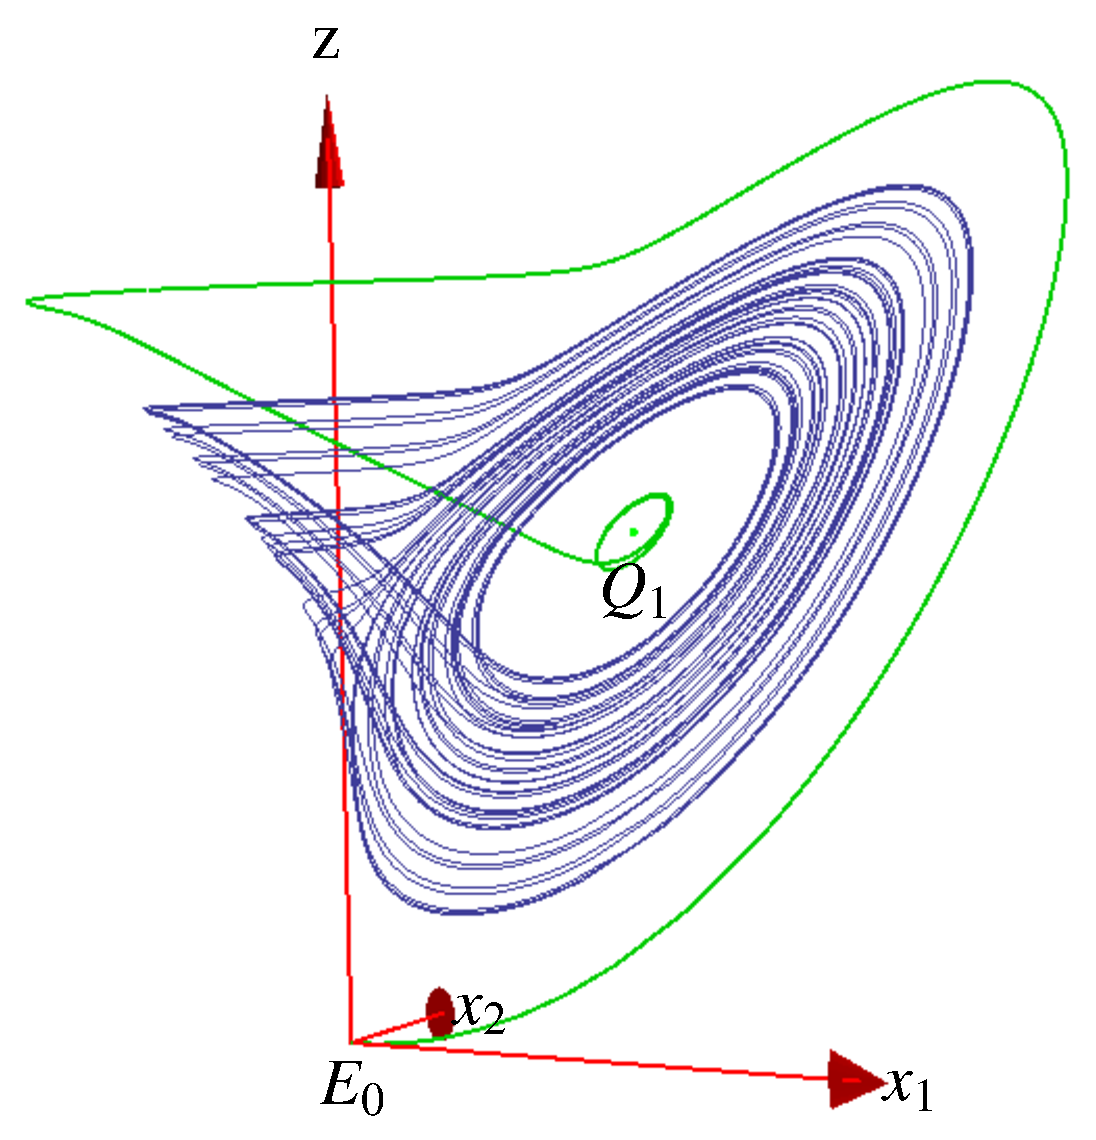
\includegraphics[width=0.43\textwidth,clip=true]{CLEperpReqb1}
~(\textit{b}) 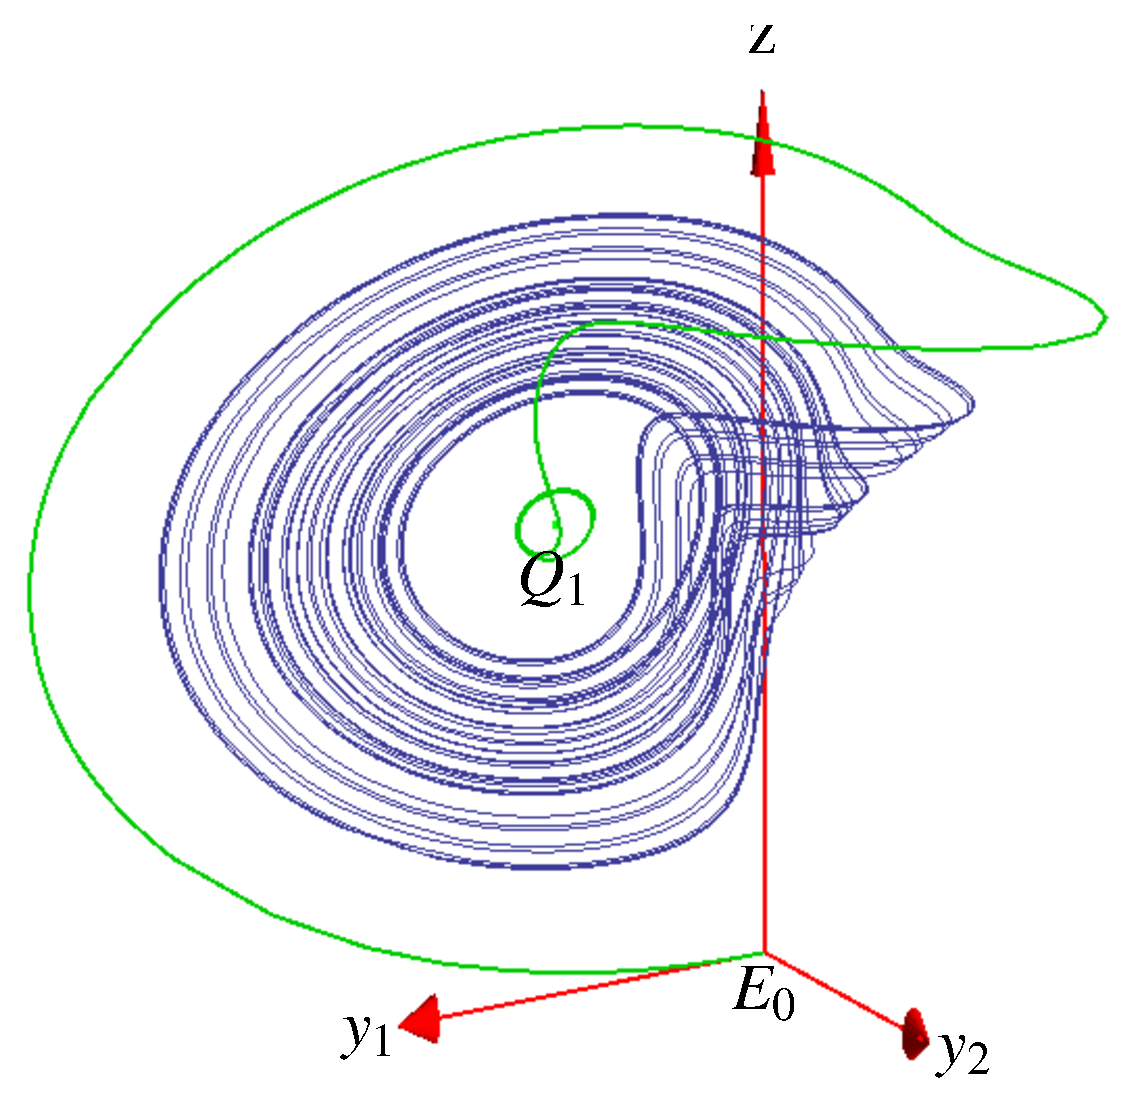
\includegraphics[width=0.43\textwidth,clip=true]{CLEperpReqb}
\end{center}
\caption{
\Statesp\ portraits of \cLe\ dynamics  in \reducedsp\
obtained by {\Mframes}, \slice\ fixed by a point on the
\reqv\ group orbit, $\slicep  = \ssp_{\REQB{1}}$.
(a) $\{x_1,x_2,z\}$ projection,
(b) $\{y_1,y_2,z\}$ projection.
}
\label{fig:CLEpcSect}
\end{figure}
%%%%%%%%%%%%%%%%%%%%%%%%%%%%%%%%%%%%%%%%%%%%%%%%%%%%%%%%%%%%%%%%
%
A long time trajectory of \refeq{EqMotionMovFramePC} with
$\slicep$ on the \reqv\ \REQB{1} group orbit is shown in
\reffig{fig:CLEpcSect}. Note that this figure is, not coincidentally,
identical to \reffig{fig:CLEmfReqb1}.
As initial condition we chose an initial point on the unstable manifold
of \REQB{1}, rotated back to the \slice\ by angle $\theta$ as
prescribed by \refeq{PCsectQ1}.
    \PC{ in \reffig{fig:CLEpcSect}:\\
        * please, no both this figure and 'coincidentally'
          \reffig{fig:CLEmfReqb1}. \Mframes\ and \mslices\ are
          \emph{identical}, former is the integral version of the latter,
          so this is an embarrassing claim. The reduced flows are of course
          one and the same for the same choice of the slice point.
          \\
        * I think it is a bad idea too plot both $\{x_1,x_2,z\}$ and
          $\{y_1,y_2,z\}$ projections. They are too tightly coupled, and
          look very much the same. That is why in ChaosBook I plot
          $\{x_1,x_2,z\}$ and
          $\{x_1,y_2,z\}$ projections; the latter exhibits the sharp
          singular space discontinuity.
        * Mark $\ssp_{\REQB{}1}$ \\
        * Draw stable eigenvector of $\ssp_{\REQB{}1}$\\
        * State value of $\ssp_{\REQB{}1}$ somewhere
     {\bf ES:} Agreed. Draw stable eigenvector of $\ssp_{\REQB{}1}$? Not sure this would look
		  nice at this scale, I will instead indicate direction of motion along unstable
		manifold of \EQV{0} by arrow.}

% \PublicPrivate{}{
% % %%%%%%%%%%%%%%%%%%%%%%%%%%%%%%%%%%%%%%%%%%%%%%%%%%
% % % computed by PCunrot.nb
% % \SFIG{PCunrot1}
% % {}{
% % {\Mframes}, continuous time version, for the
% % polar coordinates motivated $x^{*}=(0,1,0,0)$,
% % $x_1=0,\;x_2>0$, \slice. The \CLf\ strange attractor of
% % \reffig{fig:CLE} exhibits a discontinuity at
% % $x_2=0$ in the \reducedsp:
% % $\{x_2,y_2,z\}$ projection.
% % }
% % {fig:PCunrot1}
% % %%%%%%%%%%%%%%%%%%%%%%%%%%%%%%%%%%%%%%%%%%%%%%%%%%
%
% Indeed, the method does encounter singularities in
% subsets of \statesp.
% For example, the \reducedsp\ equations \refeq{PCsectSin}
% for the polar coordinates inspired \slice\
% $x^{*}=(0,1,0,0)$, $x_1=0,\;x_2>0$,
% %this is illustrated by \reffig{fig:PCunrot}.
% %$(\rho_1,\theta_1)$ are polar coordinates, $\rho_1 =
% %\sqrt{\ssp_1^{ 2} + \ssp_2^{2}}$, see \refeq{eq:CartToPol},
% are given by
% \beq
% \dot{\ssp} = \vel - \frac{\vel_1}{\ssp_2} \Lg \cdot \ssp
% \,.
% \ee{EqMotionMovFrame}
% A typical trajectory is shown in \reffig{fig:PCunrot}.
%    \PC{this is not \reffig{fig:PCunrot} - copy correct fig
%        from wilczak/blog
%        }
% }

%\renewcommand{\Group}{\ensuremath{\Gamma}}    % Siminos Lie group
